% !TEX root = ./multilinear.tex
\section{Experiments}
\label{sec:experiments}
The performance study of the proposed parallel algorithms cover the following topics.

\begin{itemize}
\item 
\textbf{Strong scaling} looks at the total runtime as the number of parallel processors are increased, thereby reducing the computing workload per process.(Section \ref{sec:strong-scaling})
\item
\texbf{Weak scaling} investigates the performance variation  while keeping a constant work load per process. The overall
How does performance varies with parallelism over iterations and graph nodes? (Section~\ref{sec:n1n}
\item
How does performance of finding paths compare with the popular FASCIA~\cite{6877274} subgraph counting implementation? (Section~\ref{sec:vsfascia})
\item
How does performance compare with the popular distributed vertex programming model,
Giraph? (Section \ref{sec:compare-giraph})
%\item
%How do our methods compare with those based on color coding?
\item
What are settings where the scaling to larger subgraph size gives new results? (Section \ref{sec:traffic})
\end{itemize}

\subsection{Experimental Setup}
\subsubsection{Hardware}
Experiments were conducted on Juliet, an Intel Haswell HPC cluster. Up to 32 nodes were used for the evaluation, where each node has 36 cores (2 sockets x 18 cores each). A node consists of 128GB of main memory and 56Gbps Infiniband interconnect. We also tested on another HPC cluster, Shadowfax-Haswell, where we used 32 nodes each with 32 cores (2 sockets x 16 cores each). Memory and interconnect of this cluster are similar to those of Juliet.

\subsubsection{Datasets}
For the two applications (paths and scan statistics), we evaluate our algorithms in datasets from different domains, such as social networks, citation networks, and road networks. A summary of the datasets is provided in Table \ref{table:datasets}. All the networks may be found in the SNAP repository \cite{snapnets}. In addition, we perform experiments in two Erdos-Renyi networks of 1 and 10 million nodes with an expected number of edges of $n\log n$, where $n$ is the number of nodes.

\begin{table}[ht]
\centering \caption{\small Datasets used in our experiments}
\vspace{-.1in}
\label{table:datasets}
%\resizebox{\columnwidth}{!}{
%\begin{scriptsize}
\begin{tabular}{|l|r|r|}
\hline
\textbf{Dataset}  & \textbf{Nodes ($\times 10^6$)} & \textbf{Edges ($\times 10^6$)} \\
\hline
miami & 2.1 & 51.5\\
\hline
com-Orkut  & 3.1 & 234.3\\
\hline
random-1e6 & 1 & 13.8\\
\hline
random-1e7 & 10 & 161.8\\
\hline
\end{tabular}
%\end{scriptsize}
%}
\end{table}

\begin{figure*}[!htb]
    \centering
    \begin{minipage}{0.23\textwidth}
        \centering        
        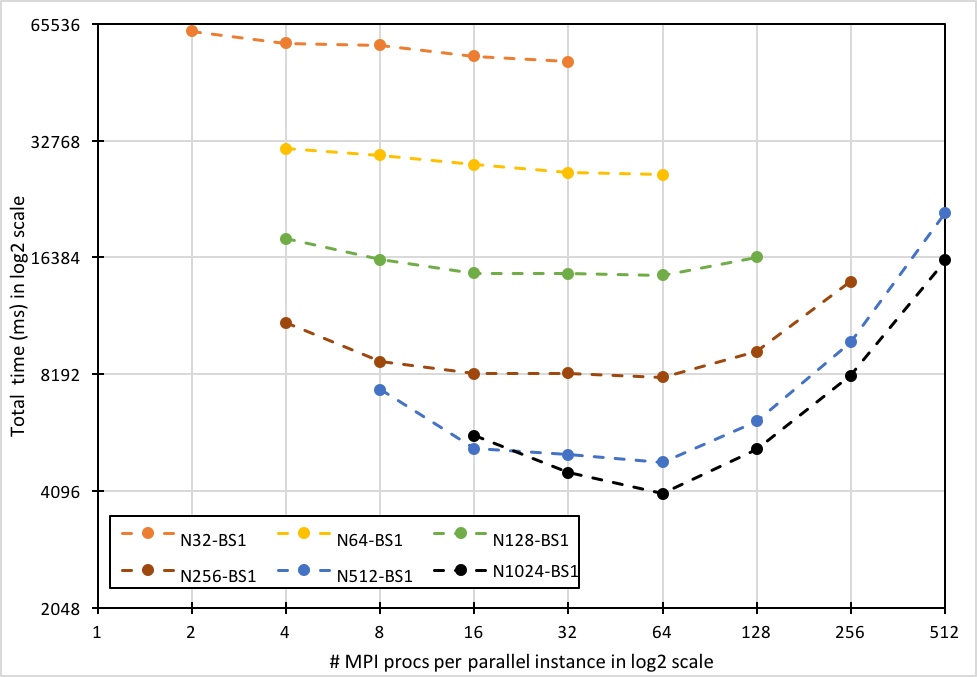
\includegraphics[width=1\columnwidth]{img/kpath-N1N/1mil-k6-BS1.png}
        \caption{\textcolor{blue}{kpath-1mil-k6-BS title}}
        \label{fig:fig-kpath-1mil-k6-BS1.png}
    \end{minipage}
    \hspace{0mm}
    \begin{minipage}{0.23\textwidth}
        \centering
        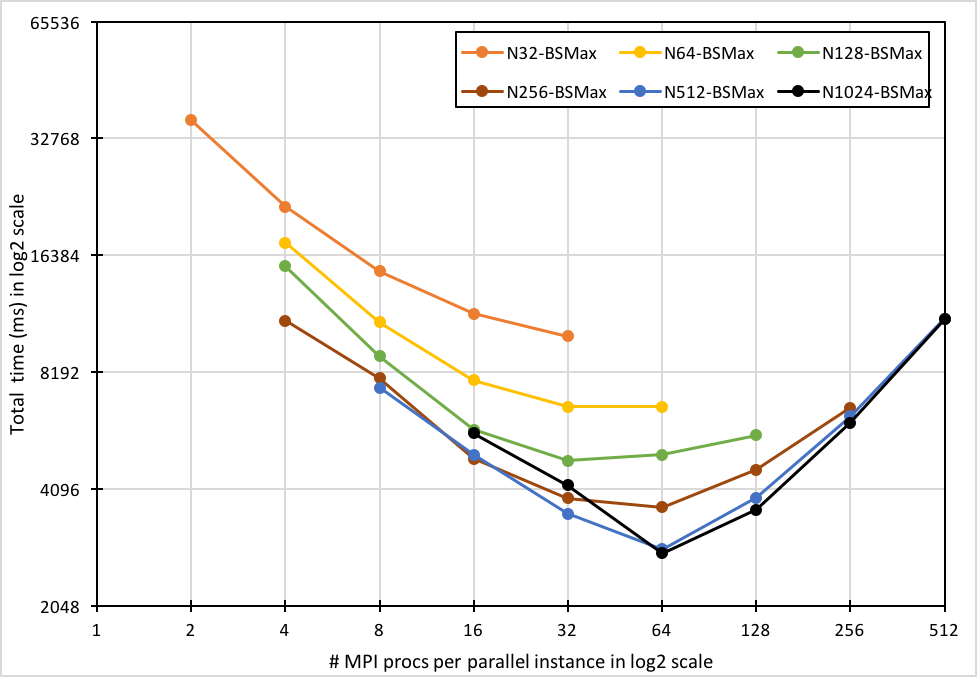
\includegraphics[width=1\columnwidth]{img/kpath-N1N/1mil-k6-BSMax.png}
        \caption{\textcolor{blue}{kpath-1mil-k6-BSMax}}
        \label{fig:fig-kpath-1mil-k6-BSMax.png}
    \end{minipage}  
    \hspace{0mm}
    \begin{minipage}{0.23\textwidth}
        \centering
        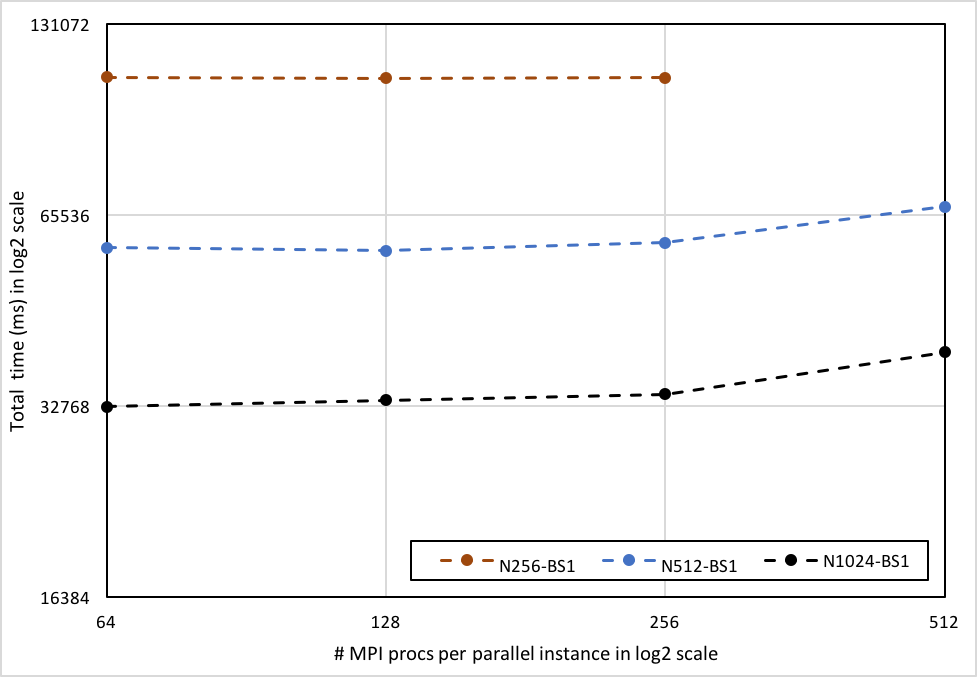
\includegraphics[width=1\columnwidth]{img/kpath-N1N/10mil-k6-BS1.png}
        \caption{\textcolor{blue}{kpath-10mil-k6-BS1}}
        \label{fig:fig-kpath-10mil-k6-BS1.png}
    \end{minipage}   
    \hspace{0mm}
    \begin{minipage}{0.23\textwidth}
        \centering
        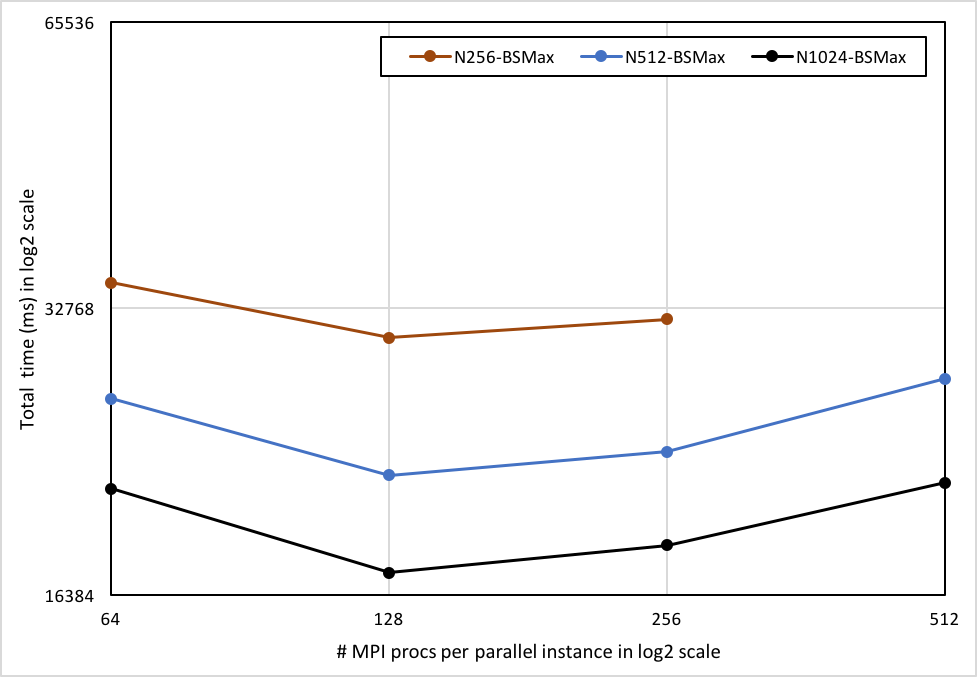
\includegraphics[width=1\columnwidth]{img/kpath-N1N/10mil-k6-BSMax.png}
        \caption{\textcolor{blue}{kpath-10mil-k6-BSMax}}
        \label{fig:fig-kpath-10mil-k6-BSMax.png}
    \end{minipage}   
    \hspace{0mm}
    \begin{minipage}{0.23\textwidth}
        \centering
        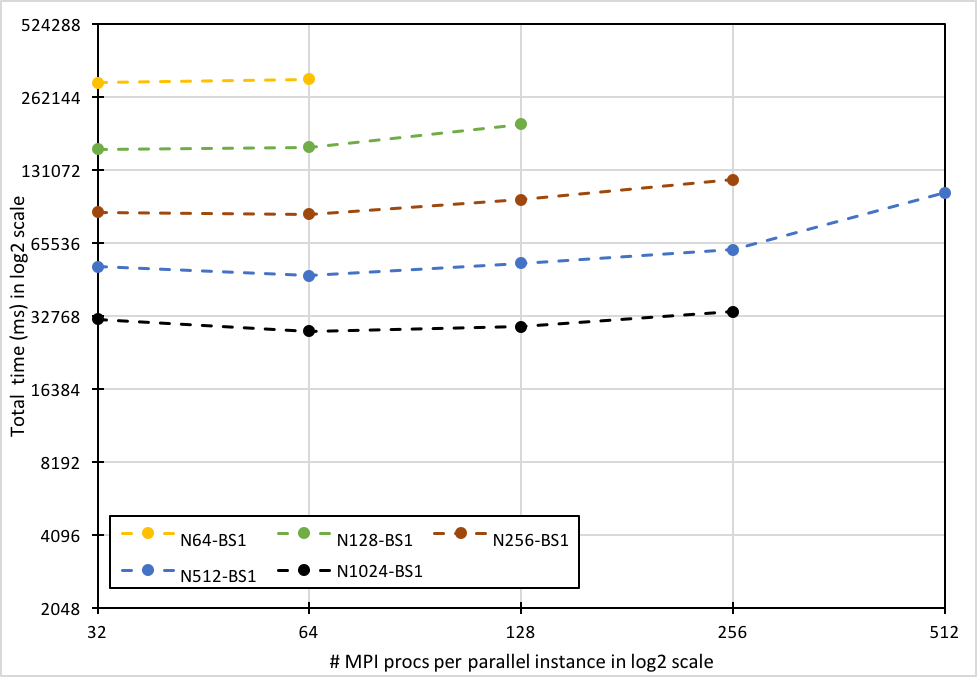
\includegraphics[width=1\columnwidth]{img/kpath-N1N/orkut-k6-BS1.png}
        \caption{\textcolor{blue}{kpath-orkut-k6-BS1}}
        \label{fig:fig-kpath-orkut-k6-BS1.png}
    \end{minipage}   
    \hspace{0mm}
    \begin{minipage}{0.23\textwidth}
        \centering
        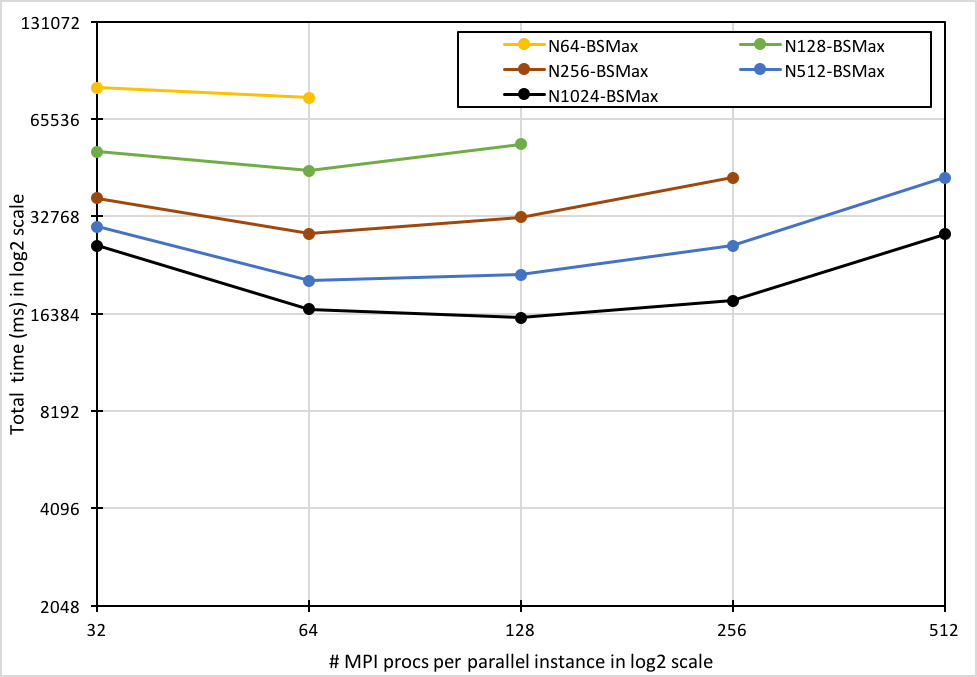
\includegraphics[width=1\columnwidth]{img/kpath-N1N/orkut-k6-BSMax.png}
        \caption{\textcolor{blue}{kpath-orkut-k6-BSMax}}
        \label{fig:fig-kpath-orkut-k6-BSMax.png}
    \end{minipage}   
    \hspace{0mm}
    \begin{minipage}{0.23\textwidth}
        \centering
        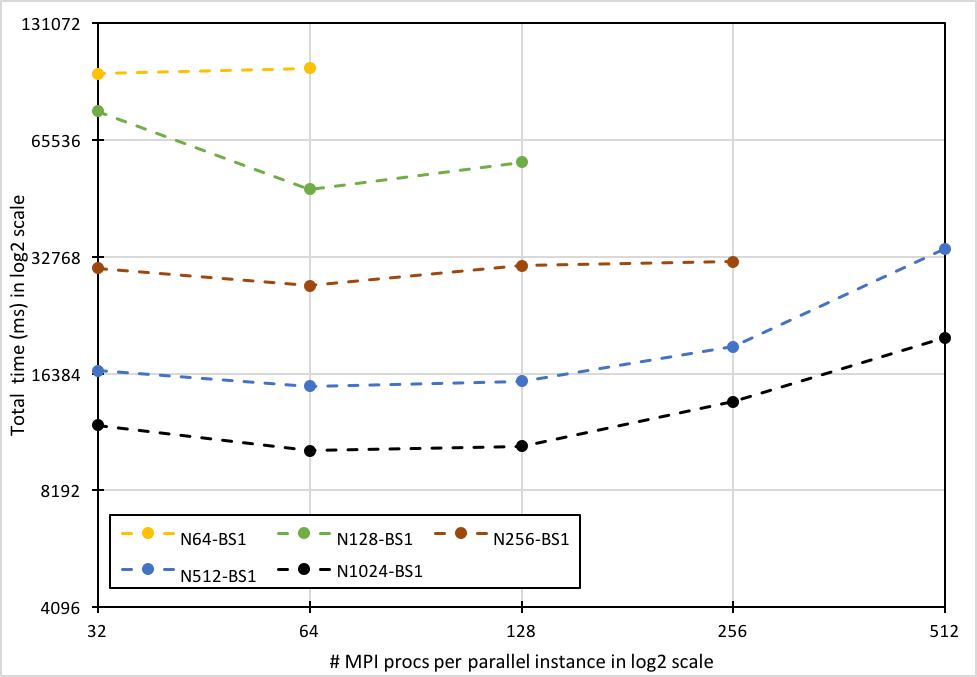
\includegraphics[width=1\columnwidth]{img/kpath-N1N/miami-k6-BS1.png}
        \caption{\textcolor{blue}{kpath-miami-k6-BS1}}
        \label{fig:fig-kpath-miami-k6-BS1.png}
    \end{minipage}   
    \hspace{0mm}
    \begin{minipage}{0.23\textwidth}
        \centering
        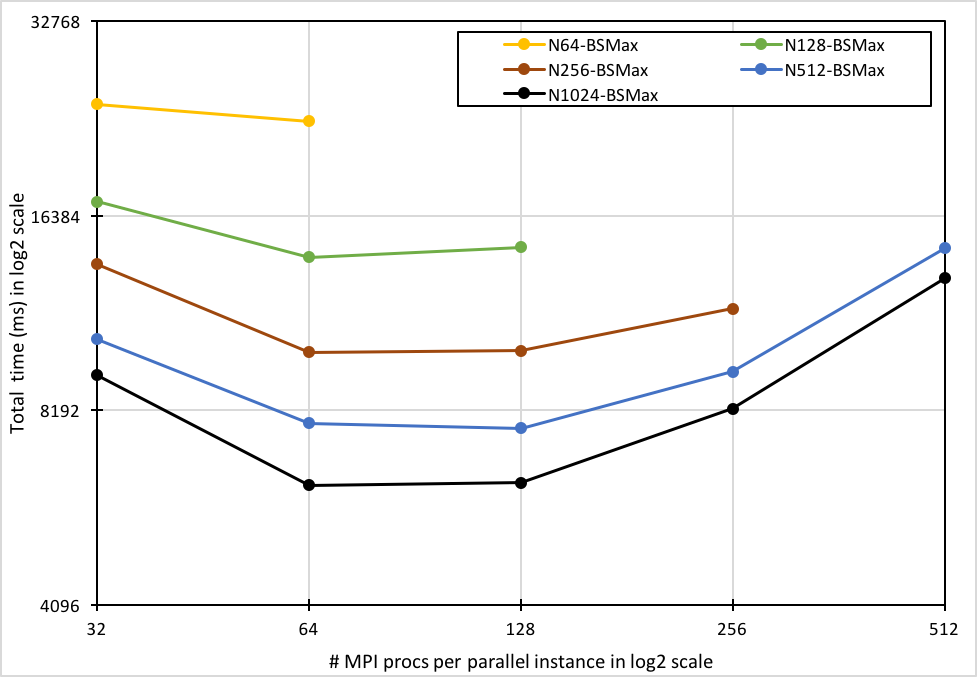
\includegraphics[width=1\columnwidth]{img/kpath-N1N/miami-k6-BSMax.png}
        \caption{\textcolor{blue}{kpath-miami-k6-BSMax}}
        \label{fig:fig-kpath-miami-k6-BSMax.png}
    \end{minipage}   
\end{figure*}

% [Saliya] I think we don't need this section on
% independence of iterations because now we don't
% run these as separate instances. Everything is 
% automatically done within the program.
% \subsection{Independence of Iterations}
% \label{sec:independence}
% First, we examine the extent to which the $2^k$ iterations of the outer loop in
% Algorithm \parmaxwt{} are independent and take the same time. Figure \ref{fig:indep} shows the running time as the number of processors $N$ is increased for the random network of 1 million nodes. This figure implies that the running time is almost invariant with the
% number of parallel iterations that are run simultaneously. We observed similar results with com-Orkut graph as shown in Figure~\ref{fig:indep-orkut}. We use this insight to estimate the total running time for other settings. 

% \begin{figure}[!htpb]
% 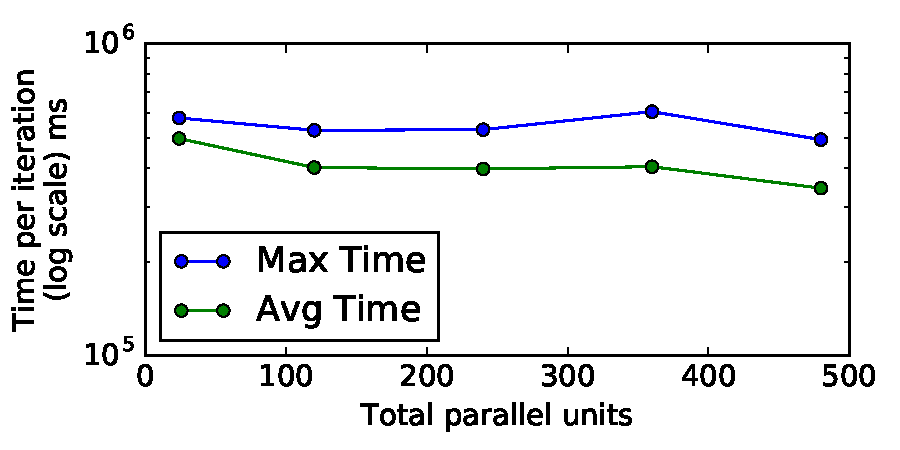
\includegraphics[width=0.4\textwidth]{img/fig-random-1mil-timeperiteration.pdf}
% \caption{Time per iteration with varying parallel units for random 1 million nodes network.}
% \label{fig:indep}
% \end{figure}

% \begin{figure}[!htpb]
% 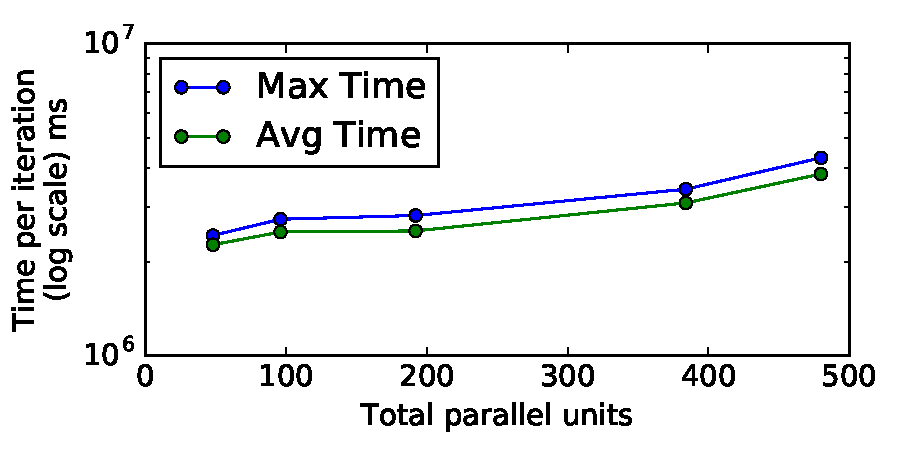
\includegraphics[width=0.4\textwidth]{img/fig-orkut-timeperiteration.pdf}
% \caption{Time per iteration with varying parallel units for Orkut network.}
% \label{fig:indep-orkut}
% \end{figure}

\subsection{Scalability with $N$ and $N_1$}
\label{sec:n1n}
The multilinear detection based parallel $k$-Path and Multilinear Scan algorithms exhibit two levels of parallelism: vertex and iterations. On one hand, the $2^k$ iterations are pleasingly parallel except a reduction at the end. The parallel vertex computation within each iteration, on the other hand, requires message passing between neighbors for $k-1$ steps. 

\textcolor{blue}{TODO - change bs to N2}

Given these two levels of parallelism and a total of $N$ processes, we can split the $2^k$ iterations among $a=\lfloor N/N_1 \rfloor$ parallel instances. Each instance decomposes the graph across $N_1$ processes and performs the $k$-Path computation in parallel for $\lfloor 2^k/a \rfloor$. To reduce the communication over computation cost, the algorithm packs a user defined $bs$ number of iterations into one computation step, so each parallel instance only has to perform $\lfloor 2^k/(a*bs) \rfloor$ compute and communication phases. 

To illustrate this with an example, consider the case of $k=6$, $N=128$, $N_1=32$, and $bs=8$. The total number of iterations is $2^k = 64$. The number of parallel instances is $128/32 = 4$. Each instances only needs to run $64/4 = 16$ iterations. Since $bs=8$, the $16$ iterations can be completed in just $16/8 = 2$ phases.

A note on $bs$: increasing this value, for example $bs=16$ in the previous case, could have finished the entire program in one compute and communicate phase. This yields to higher parallel efficiency as the overhead of communication to computation is reduced. However, it increases the message size by $bs$ factor\footnote{Increasing message size for a communication step is not necessarily a bad occurrence. Reducing number of small messages in communication may lead to increased network performance.}. Depending on the number of total processes, MPI may fail to accommodate large message sizes requiring to reduce  $bs$ such that \textcolor{blue}{TODO}. 

With these two levels of parallelism we expect to see a minimal

\textcolor{blue}{Saliya TODO - fix below}
We evaluate the total time to complete for $k$-Path and Multilinear 
Scan algorithms as a function of $N_1$, the number of processes used to run 
each of the $2^k$ circuit evaluations. With a total of $N$ processes, we can run 
$\lfloor N / N_1 \rfloor$ iterations in parallel. Figure \ref{fig:time-with-p} shows the total time for both applications varying $N$ and $N_1$. First, we note that, as $N$ becomes larger, the total running time decreases for all values of $N_1$, which is expected. Second, we obtain the best performance by assigning around 8 parallel units to process an iteration, regardless of the total parallel units.

%\subsection{Comparison with Giraph}
%We now compare our \parmaxwt{} with an implementation of Algorithm \ref{alg:multilinear-detect} in Giraph, which is a ``think like a vertex" computation framework. In Figure \ref{fig:giraph-comparison}, we show the running time of \parmaxwt{} and the Giraph implementation as a function of $k$. Giraph uses all the available parallel units for each of the $2^k$ circuit evaluation. Therefore, for a fair comparison, we report the time per iteration of both implementations---even though \parmaxwt{} runs multiple evaluations in parallel. Our MPI algorithm shows much better scalability with $k$, giving as much as 5x speed up over Giraph in the LiveJournal network.
%


% \begin{figure*}[ht]
%   \centering
%   \begin{subfigure}[b]{\textwidth}
%     \centering
%     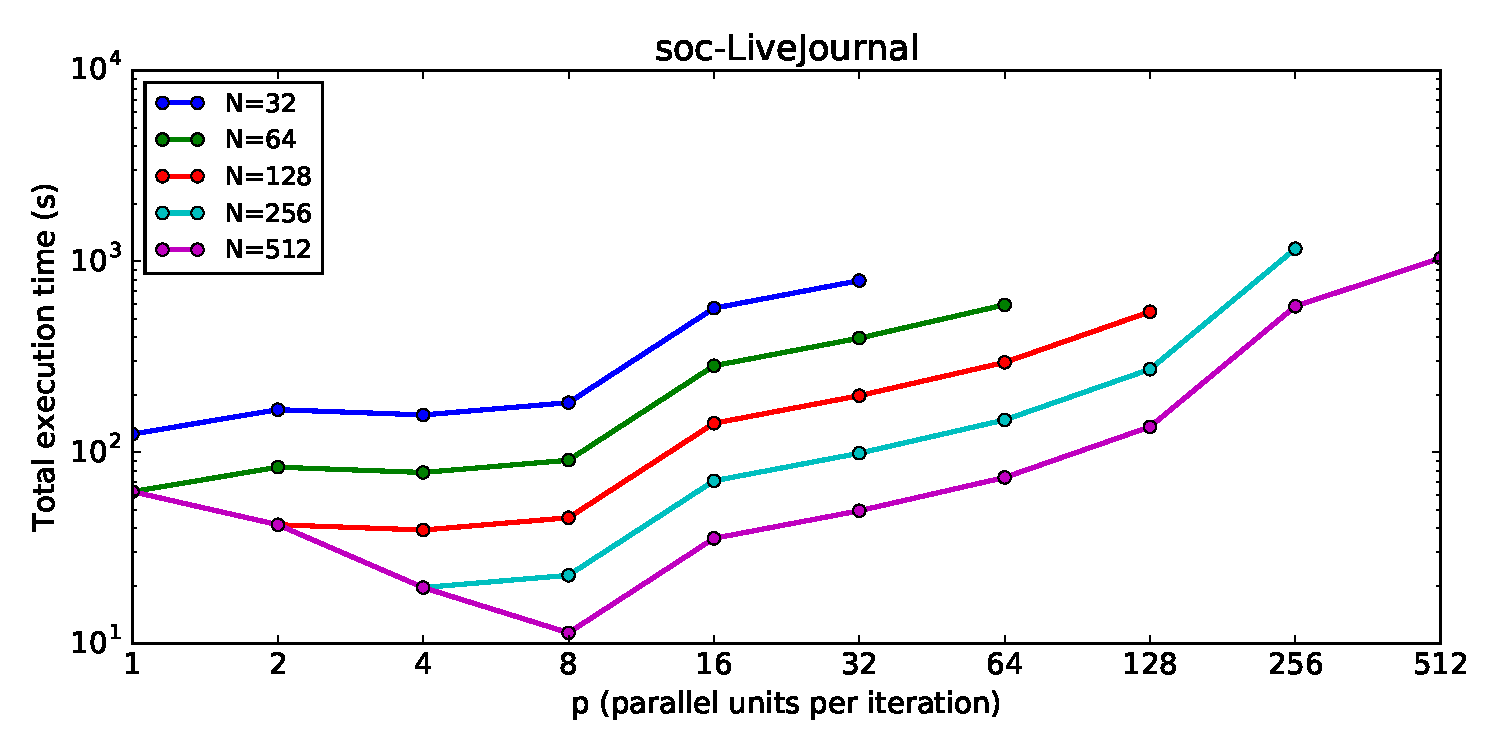
\includegraphics[width=0.49\textwidth]{img/total-time-with-p-live-journal.pdf}
%     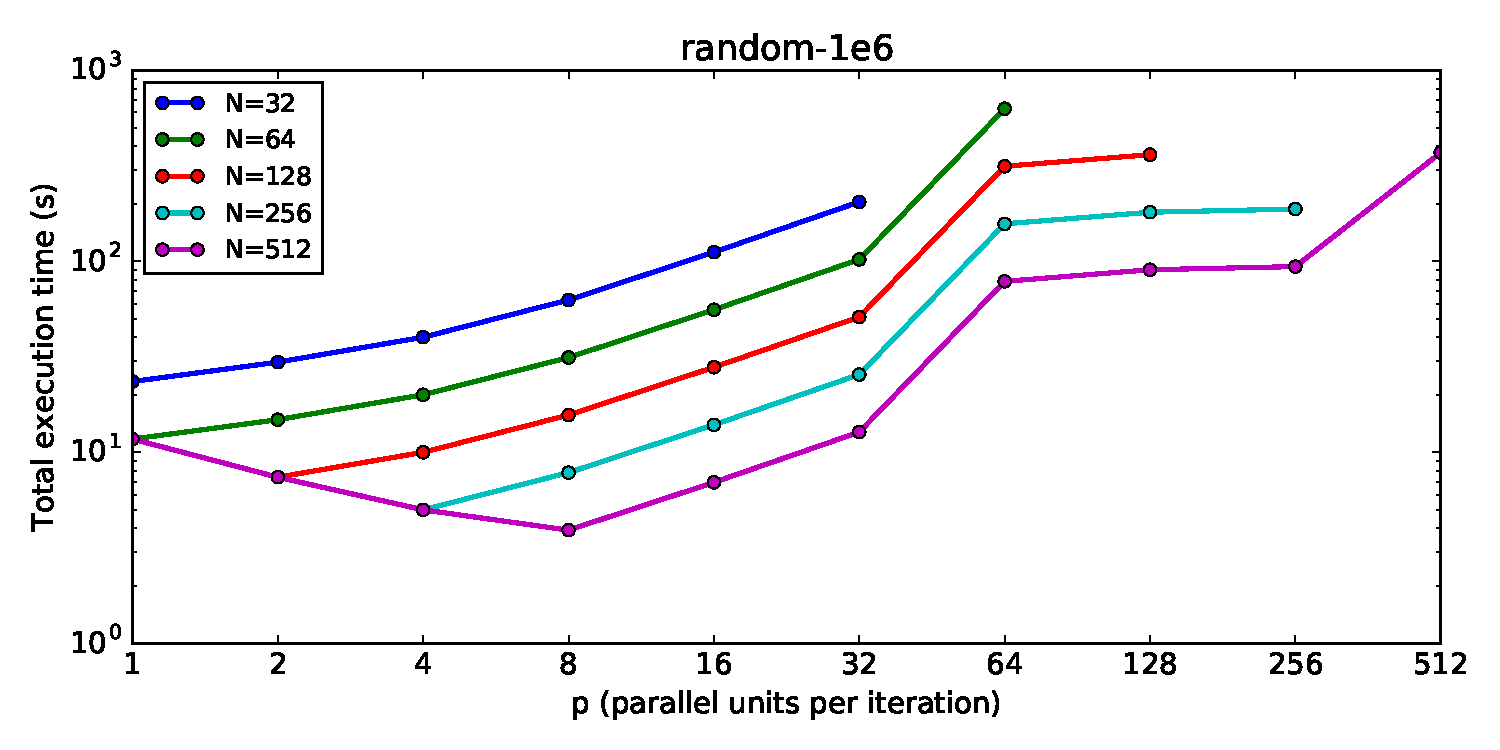
\includegraphics[width=0.49\textwidth]{img/total-time-with-p-random-er-1e6.pdf}
%     \caption{\label{fig:np-kpath} k-Path}
%   \end{subfigure}\\
  
%   \begin{subfigure}[b]{\textwidth}
%     \centering
%     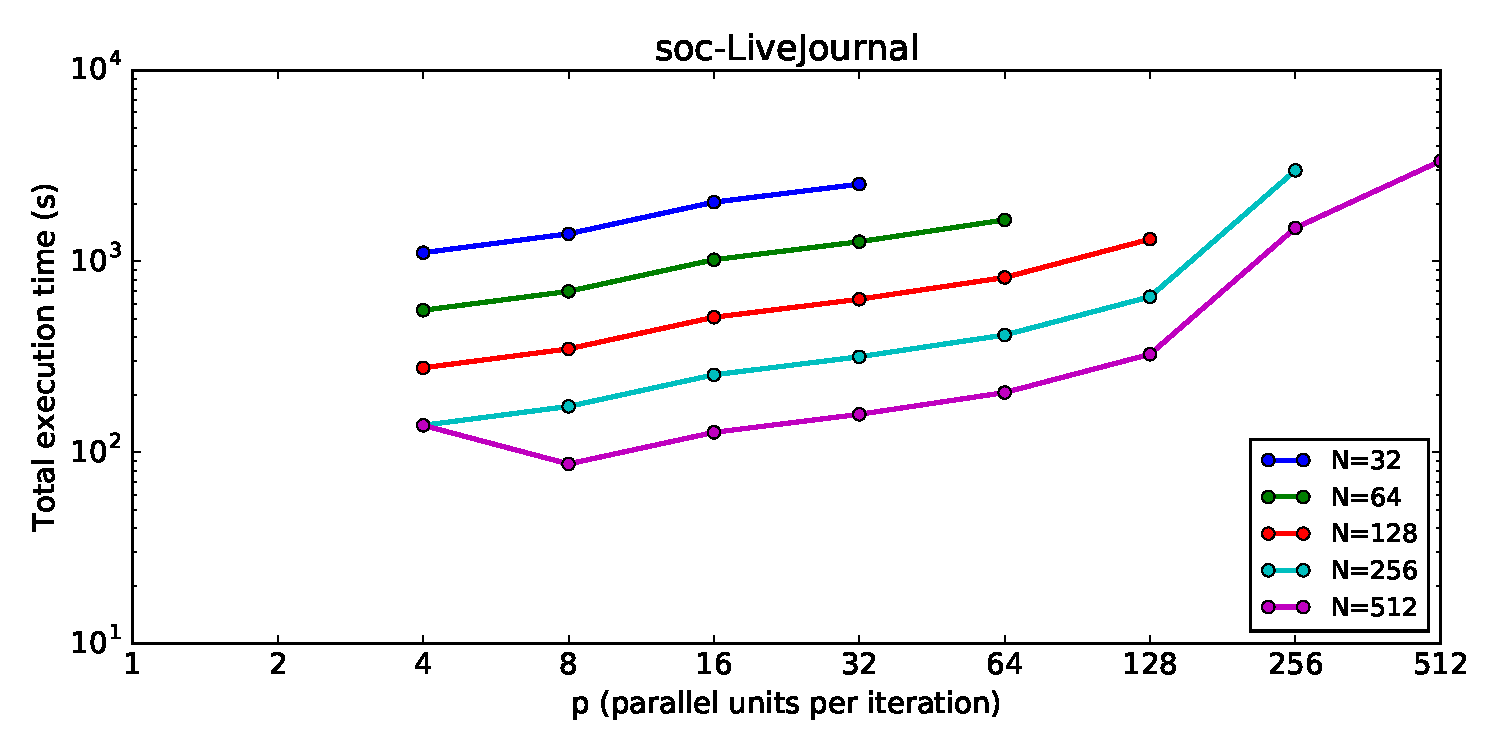
\includegraphics[width=0.49\textwidth]{img/total-time-with-p-live-journal-multilinear.pdf}
%     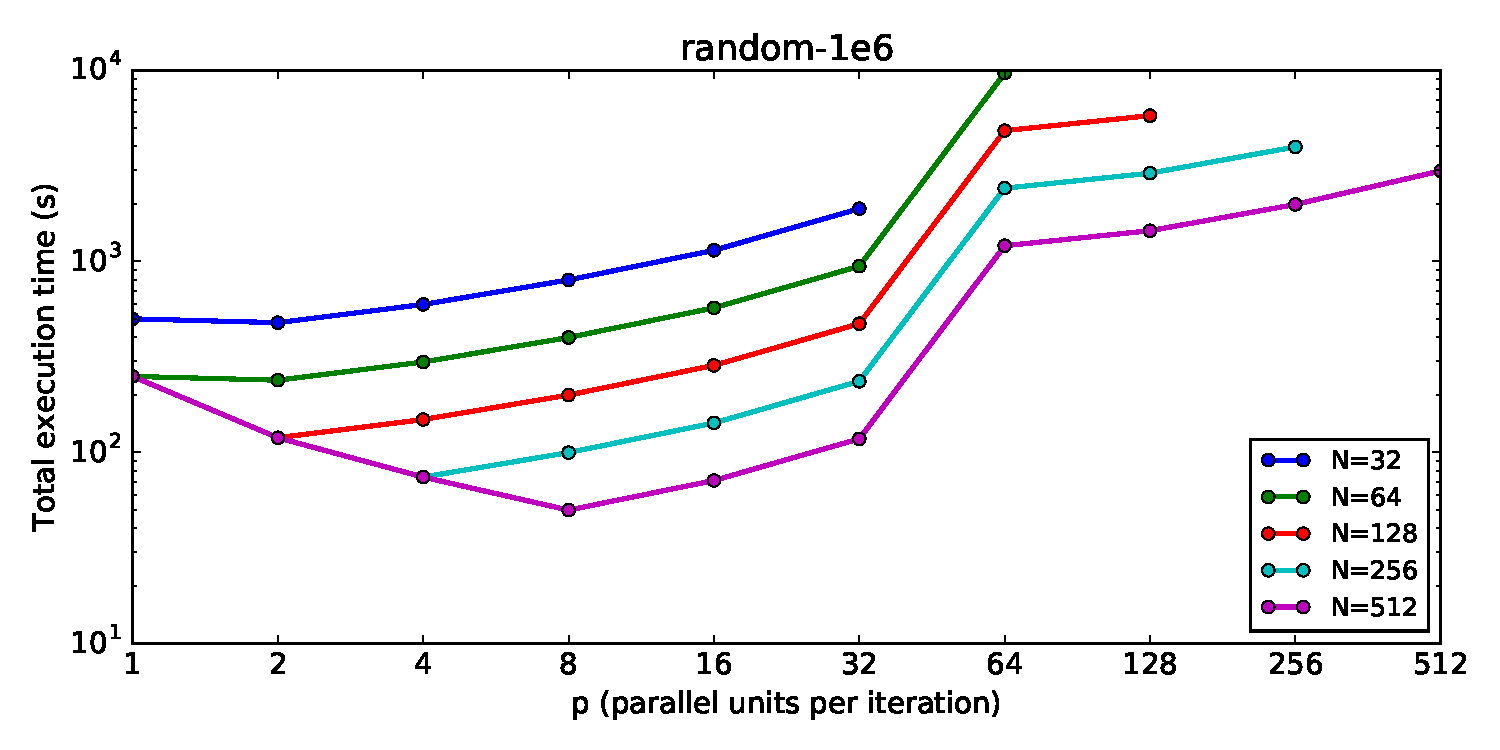
\includegraphics[width=0.49\textwidth]{img/total-time-with-p-random-er-1e6-multilinear.pdf}
%     \caption{\label{fig:np-multilinear} Multilinear Scan}
%   \end{subfigure}%
%   \caption{Scalability of our MPI algorithms for $k$-Path (\ref{fig:np-kpath}) and Multilinear Scan (\ref{fig:np-multilinear}) as a function of the total paralellism ($N$) and the units assigned to a single circuit evaluation ($p$).}
%  \label{fig:time-with-p}
% \end{figure*}

\subsection{Strong Scaling and Speedup}
\label{sec:strong-scaling}
In Figure \ref{fig:scaling}, we show the speed up and strong scaling achieved by increasing the total parallelism. We obtain higher speed up for $k$-Path, possibly because the communication overhead for this program is lower than for Multilinear Scan. In both cases, we the scaling factor is better for the LiveJournal network.

\begin{figure*}[ht]
  \centering
  \begin{subfigure}[b]{\textwidth}
    \centering
    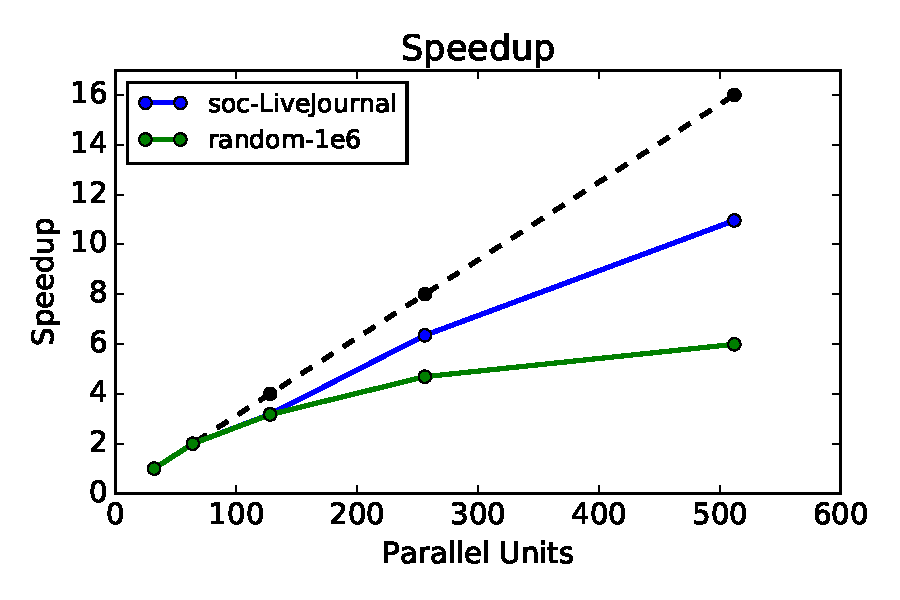
\includegraphics[width=0.45\textwidth]{img/speedup-kpath.pdf}
    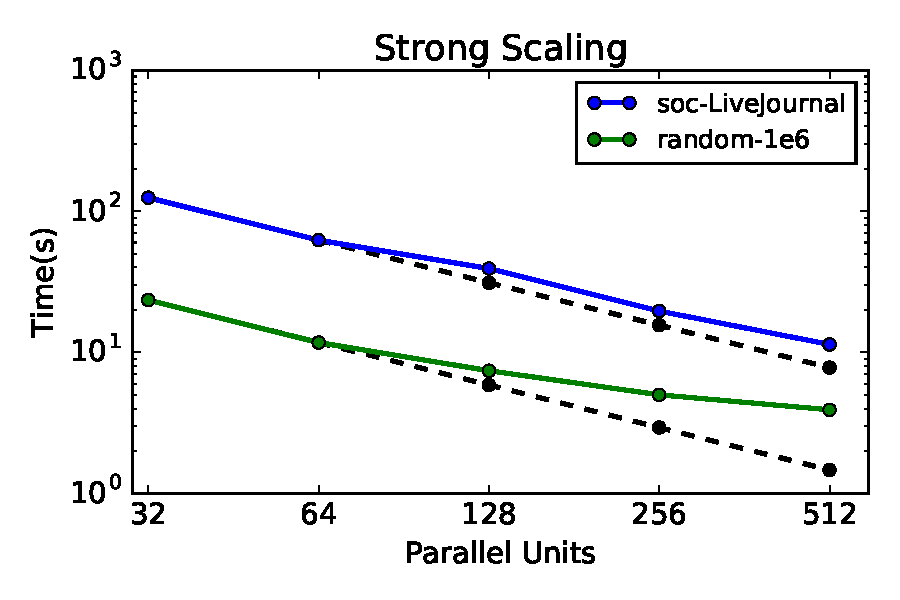
\includegraphics[width=0.45\textwidth]{img/strong-scaling-kpath.pdf}
    \caption{\label{fig:scale-kpath} k-Path}
  \end{subfigure}\\
  
  \begin{subfigure}[b]{\textwidth}
    \centering
    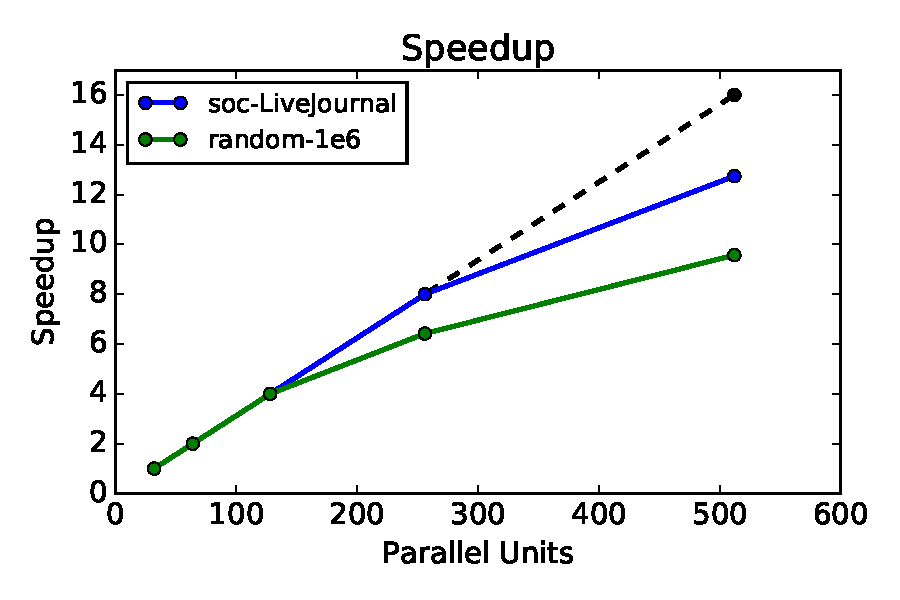
\includegraphics[width=0.45\textwidth]{img/speedup-multilinear.pdf}
    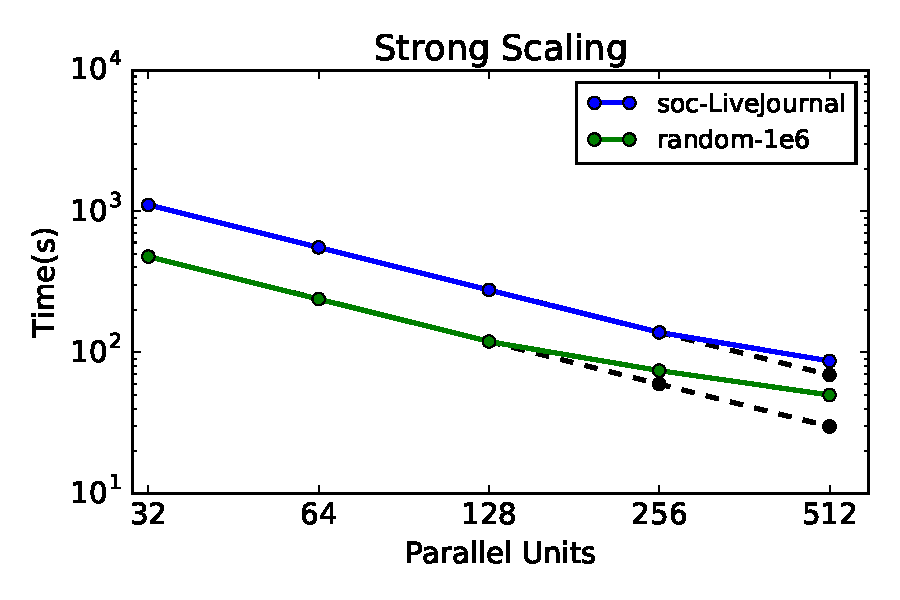
\includegraphics[width=0.45\textwidth]{img/strong-scaling-multilinear.pdf}
    \caption{\label{fig:scale-multilinear} Multilinear Scan}
  \end{subfigure}%
  \caption{Speedup and strong scaling of our MPI algorithms for $k$-Path (\ref{fig:scale-kpath}) and Multilinear Scan (\ref{fig:scale-multilinear}).}
 \label{fig:scaling}
\end{figure*}

\subsection{Comparision with Giraph}
\label{sec:compare-giraph}
%Performance for varying k=1 to k=16 in increments of 2
%This can include both random-er and snap graphs
We now compare our \parmaxwt{} with an implementation of Algorithm \ref{alg:multilinear-detect} in Giraph, which is a ``think like a vertex" computation framework. In Figure \ref{fig:giraph-comparison}, we show the running time of \parmaxwt{} and the Giraph implementation as a function of $k$. Giraph uses all the available parallel units for each of the $2^k$ circuit evaluation. Therefore, for a fair comparison, we report the time per iteration of both implementations---even though \parmaxwt{} runs multiple evaluations in parallel. Our MPI algorithm shows much better scalability with $k$, giving as much as 5x speed up  over Giraph in the LiveJournal network. We also implemented a version using Spark's GraphX library, but the communication cost associated with the dataflow model in Spark was prohibitively expensive for this algorithm. Giraph, on the other hand, follows a peer-to-peer communication model, similar to MPI, making it a better choice than GraphX.

\begin{figure}[!htpb]
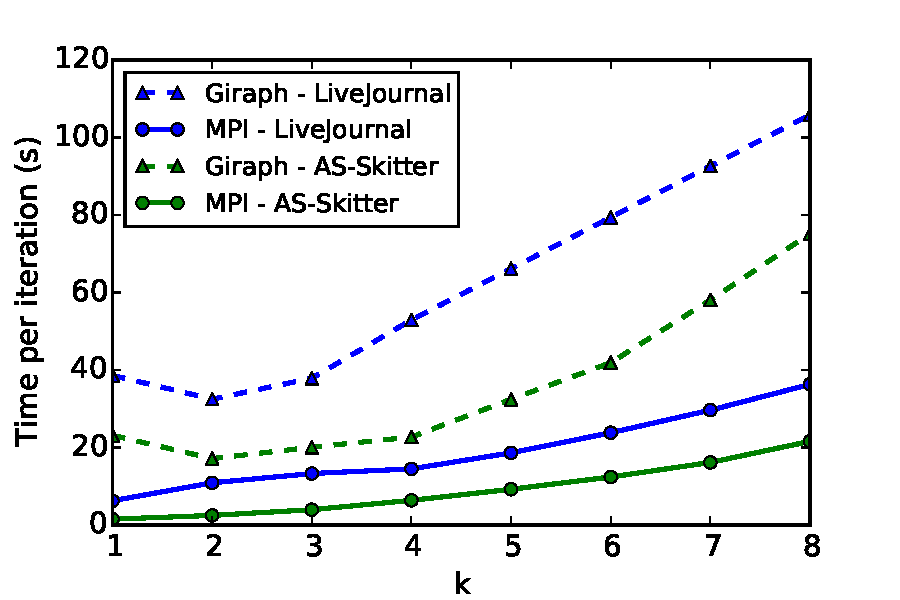
\includegraphics[width=0.4\textwidth]{img/giraph-comparison.pdf}
\caption{Running time of \parmaxwt{} as a function of $k$ compared to a Giraph implementation.}
\label{fig:giraph-comparison}
\end{figure}

\subsection{Congested Highways Clusters in Road Networks}
\label{sec:traffic}
We apply our algorithm for scan statistics to find clusters with unexpectedly low-moving traffic in the highway network of Los Angeles County\footnote{\url{http://pems.dot.ca.gov/}}. Nodes in the graph are sensors next to the road that record the average speed and the number of vehicles passing through. We have 30-minute snapshots for May 2014. We assume that the average speed recorded by each sensor follows a normal distribution. Then, the $p$-value of a node $v$ is the cumulative distribution function of a normal distribution with mean  $x_v^{[1,t-1]}$ and standard deviation $\sigma_v^{[1,t-1]}$, where $x_v^{[1,t-1]}$ and $\sigma_v^{[1,t-1]}$ are, respectively, the sample mean and standard deviation for node $v$ from snapshots $1$ to $t-1$.

We use our algorithm with $k=12$ on this dataset. In Figure \ref{fig:traffic}, we show with blue dots highway segments that our algorithm identifies as having \emph{unexpectedly} low average speed during rush hour (16:00 to 19:00) on Friday May 9, 2014. These segments are not necessarily the ones with most congestion. For instance, the center of Los Angeles city has higher congestion; however, such activity is normal on Friday afternoons according to the previous snapshots. The clusters shown in the map are selected because they have significantly lower average speeds than in previous observations.  

\begin{figure}[!htpb]
%\frame{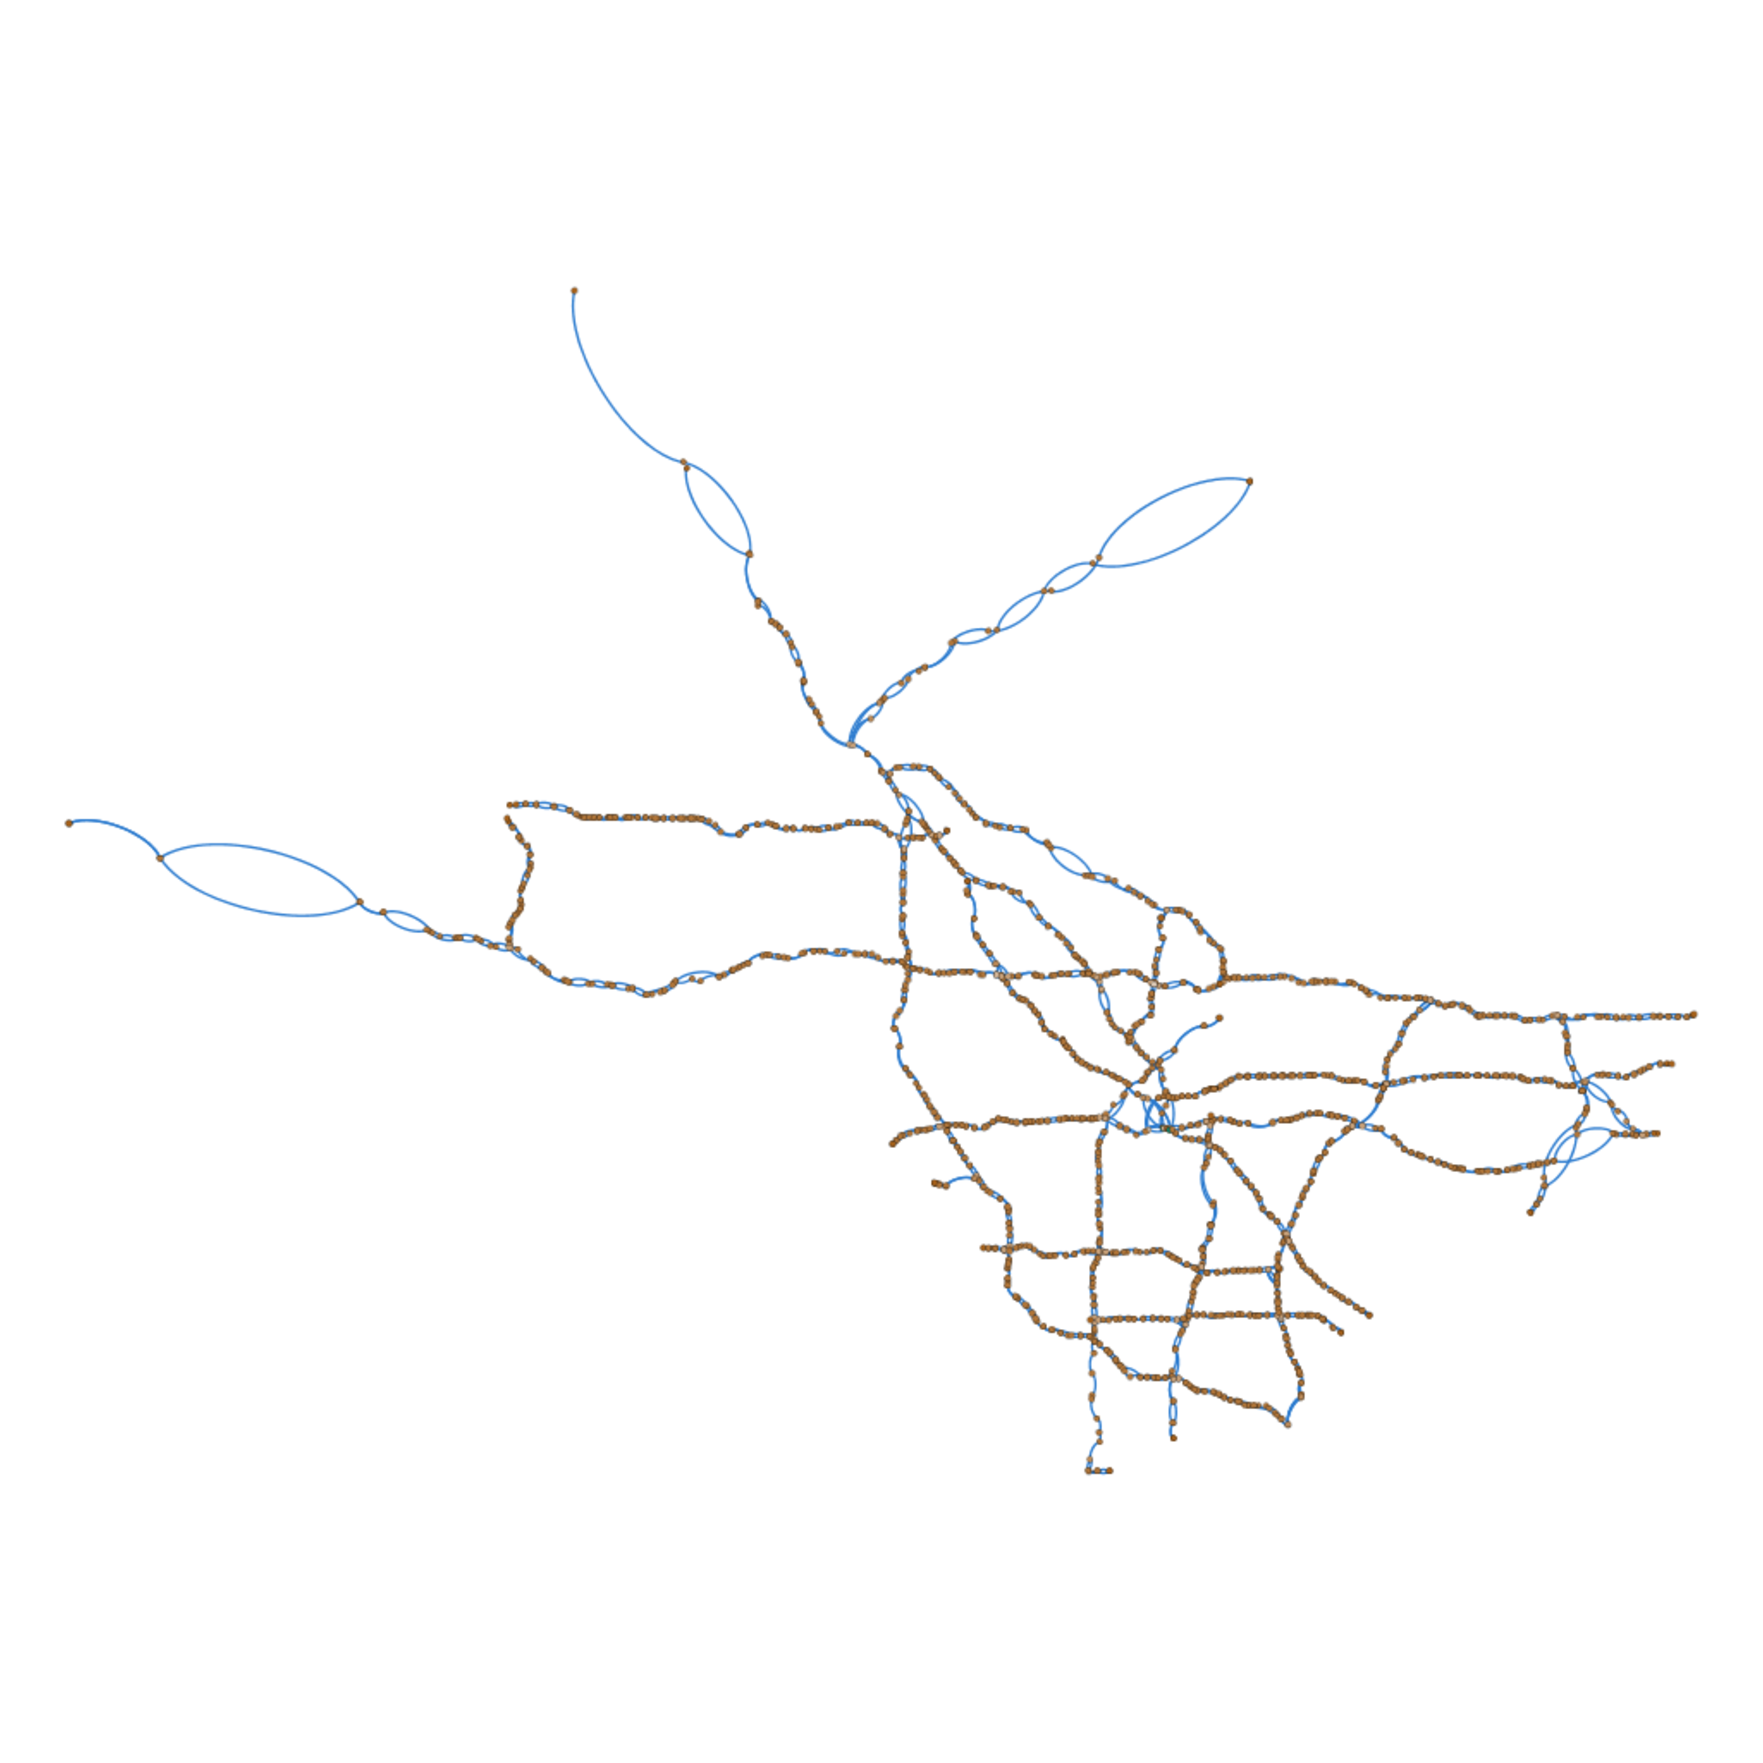
\includegraphics[width=0.48\textwidth,trim={0 4cm 0 4cm},clip]{img/traffic-network.pdf}}
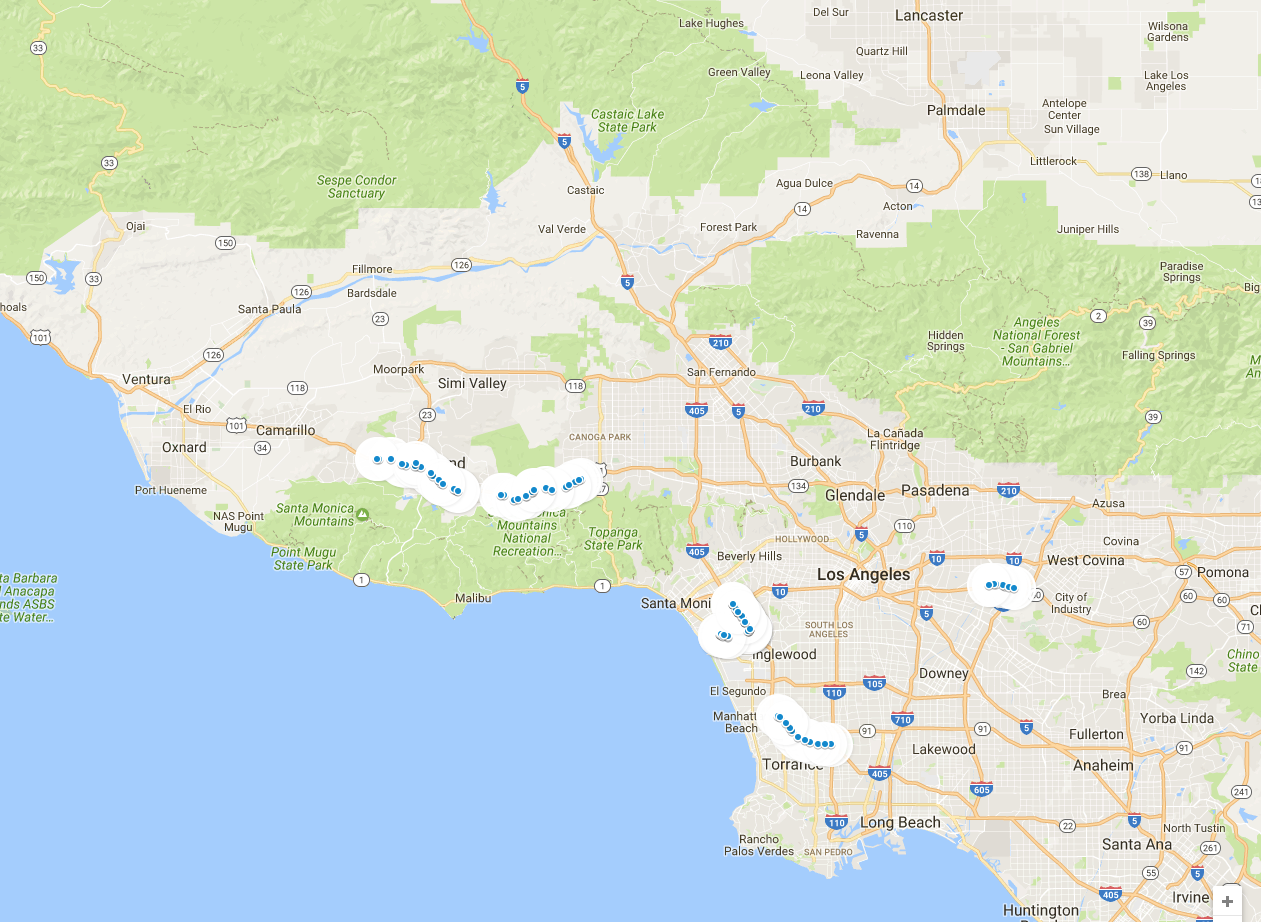
\includegraphics[width=0.48\textwidth]{img/traffic-example.png}
\caption{Discovering highway segments with unexpected congesion in the Los Angeles road network.}
\label{fig:traffic}
\end{figure}
